\documentclass[10pt, a4paper]{article}
\usepackage[utf8x]{inputenc}
\usepackage[french]{babel}
\usepackage[T1]{fontenc}
\usepackage{adjustbox}
\newcounter{nexo}           % déclaration du numéro d'exo
\setcounter{nexo}{0}        % initialisation du numero
\newcommand{\exo}[1]{
  \refstepcounter{nexo} 
  \par{{\section*{Exercice \arabic{nexo} : #1}}}\noindent}
\newcommand{\cor}[1]{
  \refstepcounter{nexo}
  \par{{\section*{Correction \arabic{nexo} : #1}}}\noindent}
\newcommand{\vv}[1]{\overrightarrow{#1}}
\newcommand{\coord}[3]{#1\begin{pmatrix}
  #2 \\
  #3
  \end{pmatrix}}
\newcommand{\coordv}[3]{\vv{#1}\begin{pmatrix}
  #2 \\
  #3
  \end{pmatrix}}
\usepackage{graphicx}
\usepackage{eurosym}
\usepackage{textcomp}
\usepackage{amsmath}
\usepackage{geometry}
\geometry{tmargin=0.6cm,lmargin=1cm,rmargin=1cm,bmargin=1.5cm}
\usepackage{xcolor}
\usepackage{dsfont}
\newcommand{\R}{\mathds {R}}
\usepackage{tikz,tkz-tab}
\usetikzlibrary{shapes.misc}
\tikzset{cross/.style={cross out, draw=red, minimum size=2*(#1-\pgflinewidth), inner sep=0pt, outer sep=0pt},
%default radius will be 1pt. 
cross/.default={1pt}}
\usepackage{pgfplots}
\pgfplotsset{compat=1.16}
\usepackage{interval}
\setlength\parindent{0pt}
\usepackage{enumitem}
%---- Style de l'entête pour le grade 10 LLG Paris-Abu Dhabi-----
%\setlength{\parindent}{0.5cm}
\newcommand{\enteteLSMI}[2]
{
  % Lieu - Année
  \noindent{\underline{\LARGE \textbf{Lycée Stendhal}} \hfill \large \textbf{Mathématiques, Classe de 4$^{\text{ème}}$}


  %  Module - Type de feuille
  \noindent{\ \ \LARGE AEFE - Milan  \large \hfill {#1}}\\
  \noindent{\phantom{Name : \dotfill}}\hfill }  
 \vspace*{-0.3cm}
  \hrule
  \begin{center} \textbf{\textsf{\Large #2 }} \end{center}\vspace*{-0.12cm}
  \hrule
  \vspace*{0.25cm}
}%
\begin{document}%

\enteteLSMI{\today}{Entrainement au contrôle sur les tableaux de signe}%

\exo{Théorème de Pythagore}%
\begin{minipage}{0.6\textwidth}%
ABC est le triangle ci-contre.\\%
AB = 8 cm\\%
BC = 11 cm.\\%
Combien mesure AC ?\\%
\end{minipage}%
\begin{minipage}{0.3\textwidth}%
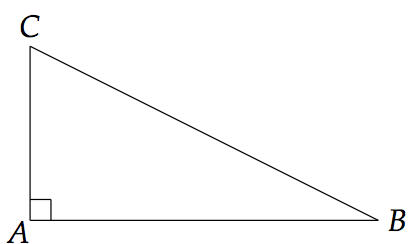
\includegraphics[width = \textwidth]{imagesQuatrieme/triangle_rectangle1.png}%
\end{minipage}%

\exo{Théorème de Pythagore}%
\begin{minipage}{0.6\textwidth}%
ABC est le triangle ci-contre.\\%
AB = 5 cm\\%
BC = 10 cm.\\%
Combien mesure AC ?\\%
\end{minipage}%
\begin{minipage}{0.3\textwidth}%
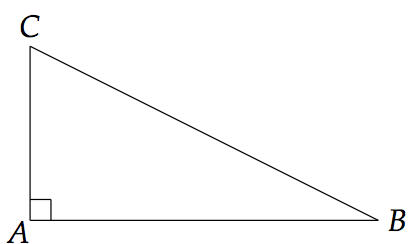
\includegraphics[width = \textwidth]{imagesQuatrieme/triangle_rectangle1.png}%
\end{minipage}%

\exo{Théorème de Pythagore}%
\begin{minipage}{0.6\textwidth}%
ABC est le triangle ci-contre.\\%
AB = 1 cm\\%
BC = 7 cm.\\%
Combien mesure AC ?\\%
\end{minipage}%
\begin{minipage}{0.3\textwidth}%
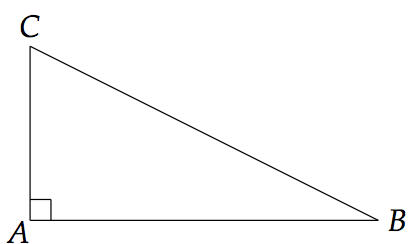
\includegraphics[width = \textwidth]{imagesQuatrieme/triangle_rectangle1.png}%
\end{minipage}%

\exo{Théorème de Pythagore}%
\begin{minipage}{0.6\textwidth}%
ABC est le triangle ci-contre.\\%
AB = 7 cm\\%
BC = 8 cm.\\%
Combien mesure AC ?\\%
\end{minipage}%
\begin{minipage}{0.3\textwidth}%
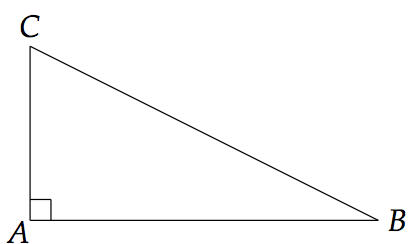
\includegraphics[width = \textwidth]{imagesQuatrieme/triangle_rectangle1.png}%
\end{minipage}%

\exo{Théorème de Pythagore}%
\begin{minipage}{0.6\textwidth}%
ABC est le triangle ci-contre.\\%
AB = 10 cm\\%
BC = 15 cm.\\%
Combien mesure AC ?\\%
\end{minipage}%
\begin{minipage}{0.3\textwidth}%
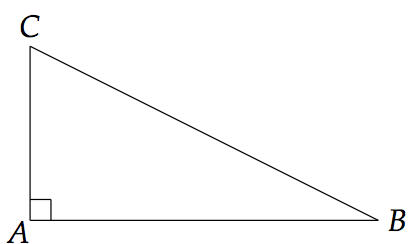
\includegraphics[width = \textwidth]{imagesQuatrieme/triangle_rectangle1.png}%
\end{minipage}%

\end{document}